\documentclass[twocolumn]{article}
\usepackage{graphicx, amssymb, amsmath, float, multicol, apacite, multirow}
\bibliographystyle{apacite}
\usepackage[a4paper, left=2.5cm, right=2.5cm, top=20mm, bottom=20mm]{geometry}
\usepackage{array}
\usepackage{changepage}
\usepackage[spanish]{babel}
\usepackage{caption}
\usepackage{subcaption}
\usepackage{diagbox}
\usepackage{footmisc}
\usepackage[hyphens]{url}  % Habilita corte de línea
\usepackage[hidelinks]{hyperref}
\usepackage{breakurl}      % permite cortar URLs largas en varias líneas
\usepackage[hyphens]{url}  % mejora los cortes en URLs
\Urlmuskip=0mu plus 1mu    % mejora la tolerancia al corte
\usepackage{algorithm}
\usepackage{algpseudocode}

\providecommand{\abs}[1]{\lvert#1\rvert}
\begin{document}
    \onecolumn
    \begin{center}
    \vspace*{0.5cm}
    {\Huge\textbf{Técnicas de condicionamiento de modelos difusivos en Cloud Removal}}
    
    \vspace{0.2cm}
    
    {\Large Lucio Luque Materazzi, Teo Manuel Kaucher}

    \vspace{0.3cm}
    
    {\Large lluquematerazzi@udesa.edu.ar \\ tkaucher@udesa.edu.ar}

    \vspace{0.3 cm}

    {\Large Ingeniería en Inteligencia Artificial}

    \Large I309 Visión Artificial Avanzada
    
    \vspace{0.5cm}

    Otoño 2026
    
    \vspace{0.5cm}

    \begin{abstract}
    En este trabajo se estudió el problema de \textit{cloud removal} sobre SEN12MS-CR, un dataset multimodal de imágenes satelitales que provee, para cada muestra, una imagen SAR, una imagen óptica nublada y su correspondiente imagen óptica libre de nubes. El objetivo principal fue analizar qué formulación difusiva resulta más adecuada para la tarea de reconstrucción y en qué medida la incorporación de información SAR mejora el resultado, evaluando distintas estrategias de fusión multimodal. Para ello se implementaron varias arquitecturas sobre una misma base U-Net, comparando la metodología clásica de un modelo difusivo, que parte de ruido gaussiano puro, con variantes que la reemplazan por un puente de difusión entre la imagen nublada y la limpia. Sobre esta última formulación se evaluaron además tres formas de introducir la información SAR: concatenación directa en la entrada, una rama auxiliar tipo ControlNet y bloques de fusión por atención cruzada mediante SARF Blocks.

    \end{abstract}


    \vspace{0.15cm}
      
\end{center}

    \begin{multicols}{2}
    \section{Introducción}
    La observación de la superficie terrestre mediante imágenes satelitales es importante en múltiples tareas de monitoreo ambiental, análisis territorial, agricultura, etc.

Sin embargo, una de las principales limitaciones de las imágenes ópticas satelitales es la presencia de nubes. En muchas ocasiones, una parte significativa de las capturas puede encontrarse parcial o totalmente cubierta por nubosidad. Esto reduce la disponibilidad de imágenes útiles y dificulta el análisis temporal de una misma región. En este contexto, la tarea de \textit{cloud removal} busca reconstruir una imagen libre de nubes a partir de una observación degradada, intentando recuperar la mayor cantidad posible de información espacial y espectral de la escena original.

El problema presenta una dificultad particular, ya que la información oculta por las nubes no se encuentra directamente disponible en la imagen óptica de entrada. En este trabajo se utiliza información SAR proveniente de Sentinel-1, ya que este tipo de sensor opera mediante radar y puede capturar características de la superficie terrestre aun en presencia de nubes, sin depender de la iluminación solar ni verse afectado de la misma forma por la nubosidad.  Sin embargo, no siempre se cuenta con este tipo de capturas, por lo que resulta relevante estudiar en qué medida la información SAR aporta o no una mejora en la reconstrucción.


% Por este motivo, resulta necesario incorporar modelos capaces de inferir contenido faltante a partir del contexto visible y, cuando es posible, aprovechar fuentes complementarias de información. En este trabajo se utiliza información SAR proveniente de Sentinel-1, ya que este tipo de sensor opera mediante radar y puede capturar características de la superficie terrestre aun en presencia de nubes. A diferencia de las imágenes ópticas, las imágenes SAR no dependen de la iluminación solar ni se ven afectadas de la misma forma por la nubosidad, por lo que constituyen una modalidad especialmente útil para complementar la reconstrucción.

En los últimos años, los modelos difusivos mostraron resultados relevantes en tareas generativas y de restauración de imágenes. Su capacidad para modelar procesos progresivos de degradación y reconstrucción los vuelve una alternativa relevante para problemas donde se busca recuperar una señal limpia a partir de una observación alterada. No obstante, en el caso específico de remoción de nubes, partir desde ruido gaussiano puro puede resultar innecesariamente costoso, ya que la imagen nublada todavía conserva parte de la estructura de la escena. Por este motivo, enfoques como DB-CR proponen formular el problema como un puente de difusión entre la distribución de imágenes nubladas y la distribución de imágenes libres de nubes.

El objetivo de este trabajo es implementar y comparar distintas arquitecturas basadas en modelos difusivos para la remoción de nubes en imágenes satelitales. Para ello, se parte de un modelo DDPM condicional y luego se desarrollan variantes inspiradas en DBCR, evaluando tanto modelos sin información SAR como distintas estrategias de incorporación multimodal. En particular, se analizan tres formas de utilizar la señal radar: concatenación directa de canales, una rama auxiliar inspirada en ControlNet y una arquitectura más compleja basada en bloques de fusión SAR-óptica mediante atención cruzada.

A lo largo del informe se describe el conjunto de datos utilizado, el marco teórico asociado a los modelos difusivos y a la formulación de \textit{diffusion bridge}, las arquitecturas implementadas, las métricas de entrenamiento y evaluación y los resultados obtenidos en cada experimento. Finalmente, se comparan las distintas variantes propuestas con el fin de analizar si la información SAR mejora la reconstrucción óptica y qué tipo de fusión resulta más efectiva bajo las restricciones computacionales del trabajo.  

    \section{Conjunto de datos}\label{sec:dataset}
    Se trabajó con el conjunto de datos SEN12MS-CR\footnote{\url{https://patricktum.github.io/cloud_removal/sen12mscr/}}, un dataset multimodal diseñado específicamente para tareas de remoción de nubes en imágenes satelitales. Este conjunto de datos contiene muestras provenientes de 175 regiones de interés (\textit{Regions of Interest}, ROI) distribuidas globalmente, capturadas durante una de las cuatro estaciones del año a lo largo de 2018.

% \begin{figure}[H]
%     \centering
%     
\includegraphics[width=0.8\textwidth]{images/triplete.png}
%     \caption{caption}
%     \label{fig:triplete}
% \end{figure}
% SI ES UNA SOLA COLUMNA!!!!!!!

\begin{figure}[H]
    \centering
    
\includegraphics[width=\columnwidth]{images/triplete.png}
    \caption{Ejemplo de triplete del dataset SEN12MS-CR. De izquierda a derecha: imagen SAR de Sentinel-1 (2 canales), imagen nublada y limpia de Sentinel-2 (13 canales).}
    \label{fig:triplete}
\end{figure}


Cada región dispone de múltiples muestras, donde cada una está compuesta por un triplete de imágenes: una imagen SAR adquirida por el satélite Sentinel-1, una imagen multiespectral de Sentinel-2 en la que se presentan nubes y su correspondiente imagen multiespectral libre de nubes como se puede observar en la figura~\ref{fig:triplete}. Estas muestras fueron obtenidas a partir de la misión Copernicus de la Agencia Espacial Europea (ESA). Dado que las imágenes nubladas y de referencia no necesariamente corresponden a la misma fecha de adquisición, pueden observarse diferencias en el estado de la vegetación entre ambas. Esto introduce cierta ambigüedad en la tarea de reconstrucción, ya que la imagen objetivo puede reflejar condiciones distintas a las presentes en la imagen de entrada.


Las imágenes de Sentinel-2 cuentan con 13 canales espectrales, que cubren el espectro visible, el infrarrojo cercano (NIR) y el infrarrojo de onda corta (SWIR): B1 (aerosol costero), B2 (azul), B3 (verde), B4 (rojo), B5, B6 y B7 (red edge), B8 (NIR), B8A (red edge), B9 (vapor de agua), B10 (cirrus), B11 (SWIR 1) y B12 (SWIR 2).


El conjunto de datos completo está compuesto por 122.218 tripletes de imágenes, donde cada muestra corresponde a un parche de 256 × 256 píxeles. Debido al gran volumen de información, el dataset ocupa comprimido aproximadamente 272 GB, lo que dificulta su manipulación y procesamiento en etapas exploratorias.

Con el objetivo de comprender la problemática y desarrollar soluciones de manera eficiente, se decidió restringir el estudio únicamente a las regiones de interés ubicadas en América del Sur. Adicionalmente, se eliminaron imágenes que no contaban con sus correspondientes contrapartes dentro del triplete o estaban corruptas.


Este preprocesamiento resultó en un subconjunto compuesto por 16 ROIs, distribuidas de la siguiente manera: 6 correspondientes al verano, 3 al otoño, 3 al invierno y 4 a la primavera. Como resultado, el conjunto de datos final utilizado en este trabajo quedó conformado por 11.084 tripletes (33.252 imágenes), ocupando un espacio total de 40.8 GB.


Debido al costo computacional asociado a procesar las 13 bandas espectrales completas, la mayor parte de los experimentos se realizó con un subconjunto de 6: B2, B3, B4, B8, B11 y B12. Esta selección combina bandas visibles, infrarrojo cercano y SWIR, permitiendo conservar información relevante sobre color, vegetación, humedad y suelo. A su vez, los canales descartados aportan información redundante o poco útil para la reconstrucción: B1, B9 y B10 son bandas atmosféricas que no describen la superficie, incluso B10 presenta valores dos órdenes de magnitud menores al resto comportándose casi como un canal constante. Por otro lado, B5, B6, B7 y B8A son de red edge, solapándose espectralmente con B8. Posteriormente, para verificar empíricamente esta hipótesis, se realizó un experimento utilizando los 13 canales completos.


En cuanto a la partición de los datos, se reservó una ROI de cada estación como conjunto de test, quedando las 12 ROIs restantes para entrenamiento. Dada la limitada cantidad de ROIs, no se definió un conjunto de validación independiente. 

    \section{Marco teórico}
     \subsection{Modelos difusivos}

Los modelos difusivos constituyen una familia de modelos generativos que aprenden a revertir progresivamente un proceso de degradación. Se definen a partir de dos procesos. El primero, denominado \textit{forward}, es un proceso fijo y no aprendido que agrega ruido gaussiano a la imagen limpia de manera incremental a lo largo de $T$ pasos temporales, hasta que sea ruido puro. El segundo, denominado \textit{reverse}, es el que aprende la red: dada una muestra ruidosa en un paso $t$, el modelo estima el ruido que se le agregó, permitiendo retroceder un paso en la trayectoria.

El proceso forward permite obtener directamente la muestra ruidosa en cualquier paso $t$ a partir de la imagen limpia $\mathbf{y}_0$, sin necesidad de simular los pasos intermedios:
\begin{equation}
    \mathbf{y}_t = \sqrt{\bar{\alpha}_t}\,\mathbf{y}_0 + \sqrt{1-\bar{\alpha}_t}\,\epsilon, \qquad \epsilon \sim \mathcal{N}(0,I)
    \label{eq:forward}
\end{equation}
donde $\bar{\alpha}_t \in [0,1]$ es un coeficiente acumulado que controla cuánta señal original se conserva en el paso $t$. La trayectoria que sigue $\bar{\alpha}_t$ a lo largo de los $T$ pasos queda determinada por el \textit{noise scheduler}, que define así qué tan rápido se destruye la información de la imagen.


\begin{figure}[H]
    \centering
    
\includegraphics[width=\columnwidth]{images/ddpm_noise.png}
    \caption{Efecto del scheduler sigmoidal sobre una imagen a lo largo del proceso forward, de $t=0$ (izquierda) a $t=T$ (derecha).}
    \label{fig:ddpm_noise}
\end{figure}

En este trabajo se utilizó un scheduler sigmoidal, cuyo efecto sobre la imagen a lo largo del proceso forward puede observarse en la figura~\ref{fig:ddpm_noise}. Esta elección se basa en lo reportado por Guo et al.\footnote{\url{https://arxiv.org/pdf/2502.04669}}, quienes analizan distintas estrategias de planificación de ruido y señalan que el scheduler sigmoideo puede resultar favorable en imágenes de alta resolución frente a alternativas como el lineal o el coseno. Es consistente además con lo observado en DiffCR\footnote{\url{https://arxiv.org/pdf/2308.04417}}, donde se comparan estos tres schedulers y se reporta que el sigmoideo produce una adición de ruido más suave.


Durante el entrenamiento se toma la imagen limpia, se le agrega ruido según la ecuación~\eqref{eq:forward} para un paso $t$ muestreado al azar, y la red aprende a predecir el ruido incorporado. En esta etapa la imagen nublada se utiliza como condición del modelo, de modo que el proceso de reconstrucción esté guiado por la observación óptica disponible.


\begin{algorithm}[H]
\caption{Entrenamiento de DDPM condicional} \label{alg:ddpm_train}
\begin{algorithmic}[1]
\Require Imagen nublada $\mathbf{x}$, imagen limpia $\mathbf{y}_0$, scheduler de ruido, modelo $f_\theta$
\State Muestrear un paso temporal $t \sim \mathcal{U}(1,T)$
\State Muestrear ruido gaussiano $\epsilon \sim \mathcal{N}(0,I)$
\State Obtener la imagen ruidosa con el valor acumulado $\bar{\alpha}_t$: \[ \mathbf{y}_t = \sqrt{\bar{\alpha}_t}\mathbf{y}_0 + \sqrt{1-\bar{\alpha}_t}\epsilon \]
\State Predecir el ruido: \[ \hat{\epsilon} = f_\theta(\mathbf{y}_t, t, \mathbf{x}) \]
\State Calcular la pérdida: \[ \mathcal{L} = \left\| \epsilon - \hat{\epsilon} \right\|_2^2 \]
\State Actualizar los parámetros de $f_\theta$ mediante descenso por gradiente
\end{algorithmic}
\end{algorithm} 

Durante la inferencia el proceso se invierte. El modelo parte de ruido gaussiano puro y utiliza la imagen nublada como condición para guiar los pasos sucesivos de denoising hasta obtener una reconstrucción libre de nubes.


\begin{algorithm}[H]
\caption{Inferencia de DDPM condicional} \label{alg:ddpm_inference}
\begin{algorithmic}[1]
\Require Imagen nublada $\mathbf{x}$, scheduler de ruido, modelo entrenado $f_\theta$, cantidad de pasos de inferencia $N$
\State Inicializar $\mathbf{y}_T \sim \mathcal{N}(0,I)$
\State Definir los pasos temporales de inferencia con el scheduler
\For{cada paso temporal $t$ desde $T$ hasta $0$}
\State Predecir el ruido en la muestra actual: \[ \hat{\epsilon} = f_\theta(\mathbf{y}_t, t, \mathbf{x}) \]
\State Actualizar la muestra mediante el paso inverso del scheduler: \[ \mathbf{y}_{t-1} = \text{SchedulerStep}(\mathbf{y}_t, \hat{\epsilon}, t) \]
\EndFor \State Retornar $\hat{\mathbf{y}}_0$
\end{algorithmic}
\end{algorithm}


% En su formulación clásica, el proceso de entrenamiento implica agregar ruido gaussiano a una imagen y que el modelo aprenda a estimar ese ruido, mientras que en la inferencia se realiza el proceso inverso, se aprende a eliminar ruido paso a paso para recuperar una imagen coherente. 


% En tareas de generación de imágenes, este mecanismo permite modelar distribuciones complejas y producir resultados de alta calidad.

La principal ventaja de los modelos difusivos frente a otros enfoques generativos es su capacidad para producir reconstrucciones de mayor fidelidad y con mejor preservación de detalles finos. Sin embargo, también presentan limitaciones importantes. El proceso de muestreo puede ser costoso, ya que requiere múltiples pasos de denoising, y el entrenamiento suele demandar una cantidad considerable de datos y recursos computacionales. Además, cuando se parte de ruido puro, el camino entre la entrada degradada y la imagen limpia puede resultar innecesariamente largo para una tarea de restauración, porque la imagen nublada ya contiene información útil de la escena.


Esta última observación motiva el uso de variantes más específicas para cloud removal como DB-CR, que busca adaptar la potencia de los modelos difusivos al problema particular de la remoción de nubes.


\subsection{DB-CR}\label{sec:dbcr paper}

DB-CR, o \textit{Diffusion Bridges for Cloud Removal}\footnote{\url{https://arxiv.org/pdf/2504.03607}}, plantea una diferencia conceptual importante respecto de los modelos difusivos clásicos.

A diferencia del DDPM condicional, DB-CR no entrena al modelo para predecir el ruido agregado (algoritmo~\ref{alg:ddpm_train}), sino para estimar directamente la imagen limpia a partir de un estado intermedio del puente entre la imagen limpia y la imagen nublada.


Para un paso temporal $t$, el estado intermedio del puente se construye interpolando linealmente entre la imagen limpia y la imagen nublada:
\begin{equation}
    \mathbf{x}_t = (1-\lambda_t)\,\mathbf{y}_0 + \lambda_t\,\mathbf{x}
    \label{eq:bridge}
\end{equation}
donde $\lambda_t \in [0,1]$ es el coeficiente del puente, definido mediante un scheduler sigmoidal. A diferencia de $\bar\alpha_t$ en la ecuación~\eqref{eq:forward}, que pondera la imagen limpia frente al ruido gaussiano, $\lambda_t$ pondera la imagen nublada: vale $\lambda_0 \approx 0$ en el extremo limpio y $\lambda_T \approx 1$ en el extremo degradado. El proceso no introduce ruido en ningún momento, la trayectoria conecta directamente ambas distribuciones.


\begin{algorithm}[H]
\caption{Entrenamiento de DB-CR}
\label{alg:dbcr_train}
\begin{algorithmic}[1]
\Require Imagen nublada $\mathbf{x}$, imagen limpia $\mathbf{y}_0$, scheduler de ruido, modelo $f_\theta$
\State Muestrear un paso temporal $t \sim \mathcal{U}(1,T)$
\State Calcular el coeficiente del puente $\lambda_t$
\State Construir la muestra intermedia:
\[
\mathbf{x}_t = (1-\lambda_t)\mathbf{y}_0 + \lambda_t\mathbf{x}
\]
\State Predecir la imagen limpia:
\[
\hat{\mathbf{y}}_0 = f_\theta(\mathbf{x}_t, t, \mathbf{x})
\]
\State Calcular la pérdida:
\[
\mathcal{L} = \left\| \mathbf{y}_0 - \hat{\mathbf{y}}_0 \right\|_1
\]
\State Actualizar los parámetros de $f_\theta$ mediante descenso por gradiente
\end{algorithmic}
\end{algorithm}

Durante la inferencia, el proceso también difiere del algoritmo~\ref{alg:ddpm_inference}, del DDPM clásico. En lugar de comenzar desde ruido gaussiano puro, DB-CR comienza desde la imagen nublada. En cada paso, el modelo predice una estimación de la imagen limpia y luego se construye un nuevo estado intermedio del puente, combinando esa predicción con la imagen nublada original. A medida que disminuye el valor de $t$, el estado intermedio se desplaza progresivamente hacia la imagen limpia estimada.

\begin{algorithm}[H]
\caption{Inferencia de DB-CR}
\label{alg:dbcr_inference}
\begin{algorithmic}[1]
\Require Imagen nublada $\mathbf{x}$, modelo entrenado $f_\theta$, scheduler de ruido, cantidad de pasos $N$
\State Inicializar $\mathbf{x}_T = \mathbf{x}$
\State Definir una secuencia descendente de pasos temporales desde $T$ hasta $1$
\For{cada paso temporal $t$}
    \State Predecir la imagen limpia:
    \[
    \hat{\mathbf{y}}_0 = f_\theta(\mathbf{x}_t, t, \mathbf{x})
    \]
    \State Calcular el paso temporal anterior $t'$
    \State Calcular el coeficiente $\lambda_{t'}$
    \State Actualizar el estado del puente:
    \[
    \mathbf{x}_{t'} = (1-\lambda_{t'})\hat{\mathbf{y}}_0 + \lambda_{t'}\mathbf{x}
    \]
\EndFor
\State Retornar $\hat{\mathbf{y}}_0$
\end{algorithmic}
\end{algorithm}

\begin{figure}[H]
    \centering
    
\includegraphics[width=\columnwidth]{images/dbcr_noise.png}
    \caption{Estados intermedios del diffusion bridge entre la imagen nublada y la imagen limpia, construidos con un scheduler sigmoidal.}
    \label{fig:dbcr_noise}
\end{figure}


La motivación detrás de DB-CR es que, en cloud removal, no resulta necesariamente óptimo destruir toda la información de la imagen y reconstruirla desde ruido. La imagen nublada contiene estructuras visibles y contexto geográfico que pueden ser aprovechados durante la restauración. Por eso, el puente de difusión busca modelar una trayectoria más directa entre la imagen degradada y la imagen limpia como se puede observar en la figura~\ref{fig:dbcr_noise}.


DB-CR también utiliza las imágenes SAR para obtener información de la superficie terrestre aun en presencia de nubes. Para esto propone una arquitectura multimodal con ramas diferenciadas para extraer características de cada modalidad y bloques específicos de fusión entre SAR y óptico.


\subsection{Implementaciones}

%Una opcion es que implementaciones sea una seccion aparte de marco teorico.

Para este trabajo se implementaron distintas arquitecturas, que se describen en las siguientes secciones y que luego serán utilizadas para comparar los resultados experimentales. Todas las variantes comparten una misma estructura general de tipo U-Net, compuesta por tres bloques de reducción de resolución, dos bloques intermedios y tres bloques de reconstrucción. Esta base permite mantener una estructura similar y comparable, diferenciándose en el tipo de proceso difusivo, los bloques internos utilizados y la forma de incorporar la información SAR.
\subsubsection{DDPM condicional}\label{sec:DDPM condicional}
\begin{figure}[H]
    \centering
    
\includegraphics[width=\columnwidth]{images/DDPM.png}
    \caption{Arquitectura DDPM condicional.}
    \label{fig:DDPM}
\end{figure}
La primera arquitectura implementada, corresponde a un modelo DDPM condicional con bloques residuales, como se puede observar en la figura~\ref{fig:DDPM}. Esta arquitectura sigue el algoritmo de entrenamiento (\ref{alg:ddpm_train}) e inferencia (\ref{alg:ddpm_inference}) de un modelo difusivo clásico.  


\subsubsection{DBCR-S}
A lo largo de este trabajo, se utiliza la notación DBCR (sin guion) para referirse a las variantes propias implementadas a partir del esquema DB-CR. Estas siguen los algoritmos~\ref{alg:dbcr_train} y~\ref{alg:dbcr_inference} para entrenar e inferir.


La segunda arquitectura implementada corresponde a una versión simplificada de DBCR, denominada DBCR-Simple, que sigue la formulación de diffusion bridge descrita en la sección~\ref{sec:dbcr paper}.

\begin{figure}[H]
    \centering
    
\includegraphics[width=\columnwidth]{images/DBCRSimple.png}
    \caption{Arquitectura DBCR simple.}
    \label{fig:DBCRSimple}
\end{figure}

En términos arquitectónicos, como se puede observar en la figura~\ref{fig:DBCRSimple}, el modelo mantiene la estructura U-Net, pero reemplaza los bloques residuales clásicos por bloques NAFT (\textit{Nonlinear Activation Free with Time embedding}). Estos bloques están inspirados en NAFNet\footnote{\url{https://arxiv.org/pdf/2204.04676}}, una arquitectura propuesta para restauración de imágenes que evita activaciones no lineales tradicionales y utiliza operaciones simples, como compuertas multiplicativas, para reducir complejidad computacional.

\begin{figure}[H]
    \centering
    
\includegraphics[width=\columnwidth]{images/NAFT.png}
    \caption{Estructura interna del bloque NAFT.}
    \label{fig:NAFT}
\end{figure}

La figura~\ref{fig:NAFT} muestra la estructura interna del bloque NAFT. El bloque está compuesto por dos ramas residuales: una primera rama tipo NAF, encargada de la extracción espacial de características, y una segunda rama tipo FFN convolucional. En ambas ramas se incorpora una proyección lineal del embedding temporal, lo que permite condicionar el bloque según el paso temporal del proceso difusivo.

Las ramas NAF y FFN se incorporan mediante conexiones residuales escaladas por los parámetros aprendibles $\beta$ y $\gamma$. Estos permiten controlar cuánto aporta cada rama residual a la salida del bloque. Al inicializarse en cero, el bloque comienza comportándose de manera cercana a una identidad, lo que ayuda a estabilizar el entrenamiento.


\subsubsection{DBCR-SC}\label{sec:DBCR-SC}
Como primera estrategia para incorporar información SAR, se implementó una variante basada en concatenación de canales, denominada DBCR-SC (\textit{DBCR Simple with Concatenation}). En este caso, la imagen SAR de Sentinel-1 se concatena con la imagen óptica nublada utilizada como condición del modelo. Dado que la imagen SAR cuenta con dos canales, la condición pasa de tener $C$ canales ópticos a tener $C+2$ canales.

Esta estrategia representa la forma más simple de fusión multimodal, ya que no requiere incorporar una rama adicional para procesar la información SAR. La modificación principal se concentra en la primera capa de la red encargada de procesar la condición, mientras que el resto de la arquitectura mantiene la misma estructura que DBCR Simple.

La ventaja de esta aproximación es su bajo costo arquitectónico: permite evaluar rápidamente si la información SAR aporta información útil para la reconstrucción. Para este modelo se evaluaron dos variantes de entrenamiento: inicializando todos los pesos aleatoriamente y utilizando \textit{transfer learning} a partir del modelo DBCR-S previamente entrenado sin SAR. Esto permite analizar si partir de una representación óptica ya aprendida facilita la incorporación posterior de información radar.

\subsubsection{DBCR-SCN}\label{DBCR-SCN}
\begin{figure}[H]
    \centering
    
\includegraphics[width=\columnwidth]{images/DBCRControlent.png}
    \caption{Arquitectura DBCR-SCN con rama auxiliar tipo ControlNet.}
    \label{fig:DBCRControlnet}
\end{figure}
Como segunda estrategia de incorporación SAR, se implementó una variante inspirada en ControlNet\footnote{\url{https://arxiv.org/pdf/2302.05543}}, denominada DBCR-SCN. A diferencia de DBCR-SC, donde la información SAR se concatena directamente con la condición óptica, en esta arquitectura se utiliza una rama auxiliar encargada de procesar la imagen SAR en paralelo, como se observa en la figura~\ref{fig:DBCRControlnet}.

La motivación de esta estrategia es separar el procesamiento de ambas modalidades. La U-Net principal trabaja sobre el proceso de reconstrucción óptica, mientras que la rama SAR extrae características específicas de la modalidad radar y las inyecta en distintos niveles de la red. De esta manera, el modelo puede aprovechar la información estructural provista por Sentinel-1 sin forzar una fusión temprana de canales.

En la arquitectura implementada, las características extraídas de SAR se incorporan mediante sumas en diferentes resoluciones del encoder-decoder. Esto permite que la información radar influya tanto en representaciones de bajo nivel, asociadas a detalles espaciales, como en representaciones más profundas, asociadas a la estructura global de la escena.

El entrenamiento de esta variante se realizó en dos etapas. Primero, se entrenó el modelo DBCR-S sin SAR, de modo que la U-Net aprendiera la tarea base de reconstrucción a partir de la imagen óptica nublada. Luego, se cargaron esos pesos y se congeló la U-Net principal, entrenando únicamente la rama ControlNet asociada a SAR. Esta estrategia permite evaluar si la información radar puede mejorar una reconstrucción óptica ya aprendida sin modificar los pesos del modelo base.


\subsubsection{DBCR}\label{sec:DBCR}
Finalmente, se implementó una versión más compleja de DBCR, más cercana a la arquitectura propuesta en el trabajo original. Esta variante mantiene la formulación de diffusion bridge, pero incorpora la información SAR mediante bloques específicos de fusión multimodal, denominados SARF Blocks (\textit{SAR Fusion Blocks}).

A diferencia de las variantes anteriores, donde la información SAR se incorporaba mediante concatenación temprana o a través de una ControlNet, en este caso la imagen SAR es procesada por una rama propia de extracción de características. Luego, esas características se fusionan progresivamente con las representaciones ópticas de la U-Net principal en diferentes niveles de resolución. De esta manera, el modelo no fuerza una mezcla inicial entre modalidades, ni un entrenamiento en dos etapas, sino que permite una integración gradual y multiescala de la información radar en una única etapa de entrenamiento.

\begin{figure}[H]
    \centering
    
\includegraphics[width=\columnwidth]{images/SARF.png}
    \caption{Estructura interna del bloque SARF.}
    \label{fig:SARF}
\end{figure}

Como se observa en la figura~\ref{fig:SARF}, el bloque SARF realiza una fusión basada en atención cruzada entre las características ópticas y las características SAR. En este bloque, las características provenientes de la rama óptica se utilizan para construir la consulta $Q_{opt}$, mientras que las características provenientes de la rama SAR se proyectan para obtener la clave $K_{sar}$ y el valor $V_{sar}$.

La operación central del bloque consiste en calcular una matriz de atención entre $Q_{opt}$ y $K_{sar}$. Esta matriz permite estimar qué regiones o componentes de la representación SAR resultan relevantes para complementar la reconstrucción óptica. Luego, la atención obtenida se aplica sobre $V_{sar}$, generando una representación SAR adaptada al contenido óptico que está siendo procesado por la U-Net principal.

La atención cruzada se puede escribir como:
\begin{equation}
    Att(Q_{opt}, K_{sar}, V_{sar})= \text{softmax}\left(\frac{Q_{opt}K_{sar}^{T}}{\sqrt{d}}\right)V_{sar}
    \label{eq:cross_attention}
\end{equation}

donde $d$ representa la dimensión de las características utilizadas en el cálculo de atención.


\begin{figure}[H]
    \centering
    
\includegraphics[width=\columnwidth]{images/DBCR.png}
    \caption{Arquitectura DBCR.}
    \label{fig:DBCR}
\end{figure}


La figura~\ref{fig:DBCR} muestra la arquitectura DBCR implementada. El modelo está organizado en dos ramas principales. Por un lado, la rama óptica recibe como entrada el estado intermedio del diffusion bridge junto con la imagen óptica nublada utilizada como condición. Por otro lado, la rama SAR recibe la imagen de Sentinel-1 y extrae representaciones radar en distintas escalas espaciales.

Por restricciones de cómputo, el primer SARF Block fue implementado con \textit{window attention}, inspirada en el uso de ventanas locales de Swin Transformer\footnote{\url{https://arxiv.org/pdf/2103.14030}}, en lugar de atención global. La atención global calcula relaciones entre todas las posiciones espaciales del mapa de características, por lo que su costo crece cuadráticamente con la cantidad de píxeles o tokens. En cambio, la window attention divide en ventanas locales y calcula la atención únicamente dentro de cada ventana. En esta implementación se utilizó un tamaño de ventana de $8 \times 8$, reduciendo significativamente el costo de memoria y cómputo en el nivel de mayor resolución de la red. Esta decisión permite mantener el mecanismo de fusión por atención cruzada, aunque restringido a relaciones locales.


\subsection{Métrica de entrenamiento}
En tareas de restauración de imágenes existen diversas funciones de pérdida: algunas penalizan con mayor intensidad los errores grandes, como la MSE, mientras que otras miden errores absolutos promedio, como la MAE o L1. También existen funciones orientadas a atributos perceptuales, como la \textit{Perceptual Loss} o la pérdida adversarial.


Para este trabajo se utilizó la misma función de pérdida que en el paper original de DBCR: la MAE loss. Esta función mide el promedio de las diferencias absolutas punto a punto entre la imagen predicha y la imagen de referencia libre de nubes. En el caso de imágenes, la comparación se realiza píxel a píxel y, para imágenes multibanda, también canal a canal. Se define de la siguiente manera:

\begin{equation}
MAE=\frac{1}{mnc}\sum_{i=0}^{m-1}\sum_{j=0}^{n-1}\sum_{k=0}^{c-1}|I(i,j,k)-K(i,j,k)|
\label{eq:MAE_loss}
\end{equation}

donde $I$ y $K$ representan dos imágenes de dimensión $m \times n$ con $c$ canales.

\subsection{Métricas de evaluación}

Una vez entrenado el modelo, las métricas de evaluación buscan reportar el rendimiento del modelo sobre datos no vistos durante el entrenamiento. En las tareas de Cloud Removal se suelen utilizar las siguientes métricas específicas.

La primera métrica utilizada es la misma que se utiliza en este trabajo para el entrenamiento, MAE~\eqref{eq:MAE_loss}. En esta métrica, valores más bajos indican un mejor desempeño, ya que implican una menor diferencia promedio entre la predicción y la imagen real.

La segunda métrica es \textit{Peak Signal-to-Noise Ratio} (PSNR), que estima la relación entre la potencia máxima posible de una señal y la potencia del ruido que afecta la fidelidad de su representación. Suele expresarse en escala logarítmica en decibelios [dB] a partir del MSE, por medio de la siguiente fórmula:

\begin{equation}
    PSNR=10 \cdot log_{10}(\frac{MAX_I^{2}}{MSE}) 
    % = 20 \cdot log_{10}(MAX_I)-10 \cdot log_{10}(MSE) 
    \label{PSNR}
\end{equation}
donde $MAX_I$ es el valor máximo posible de un píxel en la imagen, siendo por lo general igual a 255 o 1 si la imagen está normalizada. En este caso, valores más altos de PSNR indican una mayor similitud entre la imagen reconstruida y la imagen de referencia.

La tercera métrica es el Índice de similitud estructural (SSIM)\footnote{\url{https://ece.uwaterloo.ca/~z70wang/publications/ssim.pdf}}. A diferencia del PSNR, que se basa únicamente en el error píxel a píxel, SSIM busca cuantificar la similitud percibida entre dos imágenes teniendo en cuenta la información estructural. Esta métrica evalúa tres componentes: estructura $s(x,y)$, luminancia $l(x,y)$ y contraste $c(x,y)$.

Dados dos parches de imagen $x$ e $y$, el SSIM se define como:
\begin{equation}
    SSIM(x,y)=[l(x,y)]^\alpha \cdot [c(x,y)]^\beta \cdot [s(x,y)]^\gamma
\end{equation}
donde comúnmente se utiliza $\alpha=\beta=\gamma=1$, lo cual simplifica la ecuación a:
\begin{equation}
    SSIM(x,y)=\frac{(2\mu_x\mu_y + C_1)(2\sigma_{xy} + C_2)}{(\mu_x^2 + \mu_y^2 + C_1)(\sigma_x^2 + \sigma_y^2 + C_2)}
    \label{SSIM}
\end{equation}
siendo $\mu_x,\mu_y$ las medias locales de los parches, $\sigma_x^2, \sigma_y^2$ sus varianzas locales, $\sigma_{xy}$ la covarianza local y $C_1, C_2$ constantes pequeñas para estabilizar la división cuando el denominador es cercano a cero. En esta métrica, valores más altos indican una mayor similitud estructural entre la imagen predicha y la imagen de referencia.

Finalmente, se utilizó la métrica \textit{Spectral Angle Mapper} (SAM), propuesta originalmente en el contexto del análisis de imágenes espectrales por Kruse et al. (1993)\footnote{\url{https://ui.adsabs.harvard.edu/abs/1993RSEnv..44..145K/abstract}}, y especialmente relevante en imágenes multiespectrales. A diferencia de MAE, PSNR o SSIM, que comparan principalmente diferencias espaciales o estructurales, SAM evalúa la similitud espectral entre dos imágenes. Para ello, considera cada píxel como un vector formado por sus valores en los distintos canales espectrales y calcula el ángulo entre el vector predicho y el vector de referencia.

\begin{equation}
\theta_{ij} =
\operatorname{arccos}\left(
\frac{I(i,j)\cdot K(i,j)}
{\|I(i,j)\|_2 \, \|K(i,j)\|_2 + \epsilon}
\right)
\label{SAM_theta}
\end{equation}

\begin{equation}
SAM(I,K)=\frac{1}{mn}\sum_{i=0}^{m-1}\sum_{j=0}^{n-1}\theta_{ij}
\label{SAM}
\end{equation}

donde $I(i,j)$ y $K(i,j)$ son los vectores espectrales asociados al píxel $(i,j)$ de la imagen predicha y de la imagen de referencia, respectivamente; $\epsilon$ es una constante pequeña incorporada para evitar divisiones por cero. El resultado se expresa en grados. En esta métrica, valores más bajos indican una mayor similitud espectral entre la imagen reconstruida y la imagen real.


% LO DE ARRIBA LO SAQUE DE NUESTRO TP FINAL DE VISIÓN ARTIFICIAL.   
    
    \section{Desarrollo}
    
% Experimentos:
% SIN SAR
% * Finetunear lama para remover nubes. uso de mascaras MEDIO QUE ESTARIA; ES UNA VERGA PERO ESTA.✔️
% * Hacer DDPM (15 y 30 ep) ✔️ Pero hay algo mal!
% * Hacer DBCR (15 y 30 ep) ✔️

% SAR
% * Concatenar con TF (15 ep) ✔️
% Concatenar con TF (30 ep) ️OPCIONAL

% * Concatenar sin TF (30 ep) ✔️
% * Concatenar sin TF (45 ep) ✔️

% * Controlnet (15 ep) ✔️
% * Controlnet (30 ep) ✔️

% * DBCR por 15 epocas ✔️
% * DBCR por 30 epocas ✔️
% * DBCR por 45 epocas ✔️
% * DBCR por 60 epocas ✔️

% * DBCR 13 bandas ️15 epocas ✔️
% * DBCR 13 bandas ️30 epocas ✔
% * DBCR 13 bandas ️45 epocas ✔

% * Data augmentation?

% Experimentos que quedan si o si: 0
% Extra: 2

En todos los experimentos se incorporaron gradient clipping y un scheduler de learning rate para estabilizar la convergencia, utilizando un learning rate de $1\times10^{-4}$ y $T=1000$. En los experimentos para el scheduler sigmoidal se utilizó $k=25$ y $\alpha_{\min}=0.0001$ en los modelos difusivos clásicos (DDPM), generando las transiciones observadas en la figura~\ref{fig:ddpm_noise}, mientras que en los modelos diffusion bridge se utilizó $k=10$ resultando en los puentes de la figura~\ref{fig:dbcr_noise}. Salvo que se indique lo contrario, todos los entrenamientos se realizaron con un batch size de 8, y todas las redes se armaron con \texttt{base\_channels=64} y \texttt{time\_dim=128}. Asimismo, en todo experimento donde no se especifica la cantidad de canales de entrada, se utilizó el subconjunto de 6 bandas espectrales descrito en la sección~\ref{sec:dataset}, dado el alto costo computacional que implicaba procesar las 13 bandas completas y la hipótesis de que algunos canales no aportaban información relevante.

Al evaluar cada experimento, se utilizaron 10 pasos de inferencia, siguiendo el algoritmo~\ref{alg:ddpm_inference} para los modelos DDPM y el algoritmo~\ref{alg:dbcr_inference} para los modelos DBCR.

\subsection{Experimentos sin SAR}

Se entrenaron los modelos~\textbf{DDPM condicional} y~\textbf{DBCR-S} en distintas configuraciones de épocas, con el objetivo de analizar qué metodología de modelos difusivos presentaba los mejores resultados.

\subsection{Experimentos con SAR}

\textbf{DBCR-SC} La imagen SAR de 2 bandas se concatenó directamente con la condición óptica, tal como se describe en la sección~\ref{sec:DBCR-SC}.  Se entrenaron dos versiones: la primera utilizando transfer learning a partir del mejor modelo de DBCR-S, y la segunda desde cero, con el fin de evaluar el impacto de esta técnica sobre la estabilidad del entrenamiento.

\textbf{DBCR-SCN} Siguiendo el esquema de dos etapas descrito en la sección~\ref{DBCR-SCN}, se congelaron los pesos del mejor modelo de DBCR-S y se entrenó únicamente la rama ControlNet encargada de procesar la información SAR.

\textbf{DBCR} Debido a la alta complejidad computacional de este modelo, producto del mecanismo de atención cruzada entre representaciones ópticas y SAR descrito en la sección~\ref{sec:DBCR}, se incorporaron distintas optimizaciones de memoria adicionales al uso de ventanas de atención de $8 \times 8$ en el primer bloque SARF como se explicó anteriormente. En primer lugar, se empleó \textit{gradient checkpointing}, técnica que recalcula activaciones intermedias durante el \textit{backward pass} en lugar de almacenarlas, reduciendo el uso de memoria a costa de un mayor tiempo de cómputo\footnote{\url{https://arxiv.org/pdf/1604.06174}}. También se utilizó Flash Attention, una implementación optimizada del mecanismo de atención que reduce los accesos a memoria y acelera su cálculo\footnote{\url{https://arxiv.org/pdf/2205.14135}}. Finalmente, se incorporó \textit{autocast} mediante PyTorch AMP, lo que permite ejecutar operaciones en precisión mixta FP16/FP32 para reducir el consumo de memoria durante el entrenamiento\footnote{\url{https://docs.pytorch.org/docs/2.13/amp.html}}.
Aun con estas optimizaciones, fue necesario utilizar un batch size de 4, alcanzando una utilización de aproximadamente 20~GB de VRAM durante el entrenamiento. Para este modelo se entrenaron dos versiones: una utilizando las 6 bandas y otra con las 13 bandas completas de Sentinel-2.
    
    \end{multicols}
    % \newpage
    \section{Resultados}
    \begin{table}[H]
    \centering
    \begin{tabular}{lccccc}
        \hline
        \textbf{Modelo} & \textbf{Épocas} & \textbf{PSNR (dB)$\uparrow$} & \textbf{SSIM$\uparrow$} & \textbf{MAE$\downarrow$} & \textbf{SAM ($^\circ$)$\downarrow$} \\
        \hline
        DDPM condicional & 15 & 16.19 & 0.311 & 0.1293 & 49.40 \\
        DDPM condicional & 30 & 18.46 & 0.180 & 0.1046 & 48.51 \\
        DBCR-S            & 15 & \textbf{27.58} & \textbf{0.807} & \textbf{0.0313} & 12.78 \\
        DBCR-S            & 30 & 26.70 & 0.798 & 0.0339 & \textbf{11.13} \\
        \hline
    \end{tabular}
    \caption{Comparación de las métricas sobre el set de testeo de los modelos sin información SAR.}
    \label{tab:sin_sar}
\end{table}

Al analizar la tabla~\ref{tab:sin_sar} se puede concluir que el DDPM condicional clásico queda muy por debajo de DBCR-S en todas las métricas, incluso después de duplicar las épocas de entrenamiento. Más llamativo aún, su SSIM empeora al pasar de 15 a 30 épocas (0.311 a 0.180), lo que sugiere que el modelo no logra estabilizarse en ese rango de entrenamiento, probablemente porque el proceso DDPM puro parte de ruido gaussiano completo y necesita muchas más iteraciones para converger en una tarea de traducción condicional como esta. En contraste, DBCR-S alcanza un desempeño sólido ya a las 15 épocas, y extender el entrenamiento no mejora PSNR/SSIM (incluso empeora levemente), aunque sí reduce el SAM, lo que indicaría una posible saturación temprana del modelo.


\begin{table}[H]
    \centering
 
    \begin{tabular}{lccccc}
        \hline
        \textbf{Modelo} & \textbf{Épocas} & \textbf{PSNR (dB)$\uparrow$} & \textbf{SSIM$\uparrow$} & \textbf{MAE$\downarrow$} & \textbf{SAM ($^\circ$)$\downarrow$} \\
        \hline
        % DBCR-S (sin SAR)  & 15 & 27.58 & 0.807 & 0.0313 & 12.78 \\
        % DBCR-S (sin SAR)  & 30 & 26.70 & 0.798 & 0.0339 & 11.13 \\
        DBCR-SC (concat, TL)      & 15 & 26.78 & 0.792 & 0.0343 & 10.71 \\
        DBCR-SC (concat, sin TL)  & 30 & \textbf{27.82} & 0.801 & \textbf{0.0287} & \textbf{9.81}  \\
        DBCR-SC (concat, sin TL)  & 45 & 26.92 & \textbf{0.803} & 0.0327 & 12.71  \\
        DBCR-SCN (ControlNet)     & 15 & 27.28 & 0.780 & 0.0320 & 11.05 \\
        DBCR-SCN (ControlNet)     & 30 & 26.92 & 0.781 & 0.0324 & 10.94 \\
        \hline
    \end{tabular}
    \caption{Comparación de las métricas sobre el set de testeo de las estrategias de incorporación de información SAR.}
    \label{tab:sar_strategies}

\end{table}

% Al observar la tabla~\ref{tab:sar_strategies} se concluye que incorporar SAR no genera una mejora dramática en PSNR/SSIM respecto del baseline sin SAR, pero sí consistentemente reduce el SAM, lo que indica que la información SAR aporta principalmente fidelidad espectral/angular más que reducción de error pixel a pixel.

Al observar la tabla~\ref{tab:sar_strategies} se concluye que, dentro de las variantes con SAR, la concatenación directa sin transfer learning a 30 épocas es la que mejor desempeño global obtiene, superando incluso a ControlNet pese a ser una estrategia más simple. Esto podría deberse a que ControlNet, al congelar la rama principal, limita la capacidad del modelo de adaptar sus features internas a la nueva fuente de información, o a que necesitaría más épocas para aprovechar completamente la rama de control. También se observa que la versión con transfer learning (15 épocas) obtiene peor desempeño que el baseline sin SAR, lo que sugiere que la información SAR puede aportar mejoras, pero resulta más efectiva al entrenarse desde el principio.

\begin{table}[H]
    \centering
    \begin{tabular}{lcccccc}
        \hline
        \textbf{Modelo} & \textbf{Canales} &\textbf{Épocas} & \textbf{PSNR (dB)$\uparrow$} & \textbf{SSIM$\uparrow$} & \textbf{MAE$\downarrow$} & \textbf{SAM ($^\circ$)$\downarrow$} \\
        \hline
        DBCR & 6  & 15 & 26.15 & 0.786 & 0.0347 & 12.05 \\
        DBCR  & 6    & 30 & 28.12 & 0.815 & 0.0293 & 10.47 \\
        DBCR  & 6    & 45 & 28.14 & 0.830 & 0.0283 & 10.39 \\
        DBCR  & 6    & 60 & \textbf{28.45} & \textbf{0.840} & \textbf{0.0274} & 9.82 \\
        DBCR  & 6    & 75 & 28.17 & 0.837 & 0.0284 & \textbf{9.53} \\
        DBCR  & 13   & 15 & 25.62 & 0.771 & 0.0368 & 12.71 \\
        DBCR & 13 & 30 & 27.21 & 0.834 & 0.0293 & 10.89 \\
        DBCR & 13 & 45 & 25.82 & 0.775 & 0.0366 & 12.11 \\
        \hline
    \end{tabular}
    \caption{Comparación de las métricas sobre el set de testeo del modelo DBCR con 6 y 13 canales.}
    \label{tab:dbcr_bandas}
\end{table}

En la tabla~\ref{tab:dbcr_bandas} se observa que la versión de 6 canales supera a la de 13 en la mayoría de las configuraciones evaluadas, con la excepción del SSIM a 30 épocas donde obtiene un valor levemente superior (0.834 vs. 0.815). Considerando el mejor modelo de cada configuración, la versión de 6 canales domina en las cuatro métricas, lo que sustenta la hipótesis de que hay canales que no aportan o degradan la información. A su vez el desempeño con la menor cantidad de canales continúa mejorando de forma progresiva a medida que se extiende el entrenamiento (15, 30, 45 y 60 épocas), aunque con 75 épocas todas las métricas, salvo SAM, empeoran, lo que podría significar un sobreajuste al set de entrenamiento, aunque la ausencia de un conjunto de validación impide confirmarlo.

Comparando el mejor resultado de DBCR (6 canales, 60 épocas) con el mejor modelo con SAR de la tabla~\ref{tab:sar_strategies} (DBCR-SC sin TL a 30 épocas), DBCR logra superarlo en PSNR (28.45 vs.\ 27.82 dB), SSIM (0.840 vs.\ 0.801) y MAE (0.0274 vs.\ 0.0287), aunque obtiene un SAM mínimamente peor (9.82 vs.\ 9.81). Esto podría indicar que el mecanismo de fusión por atención cruzada entre las características ópticas y SAR permite una reconstrucción global de mayor calidad que la simple concatenación.


\begin{figure}[H]
    \centering
    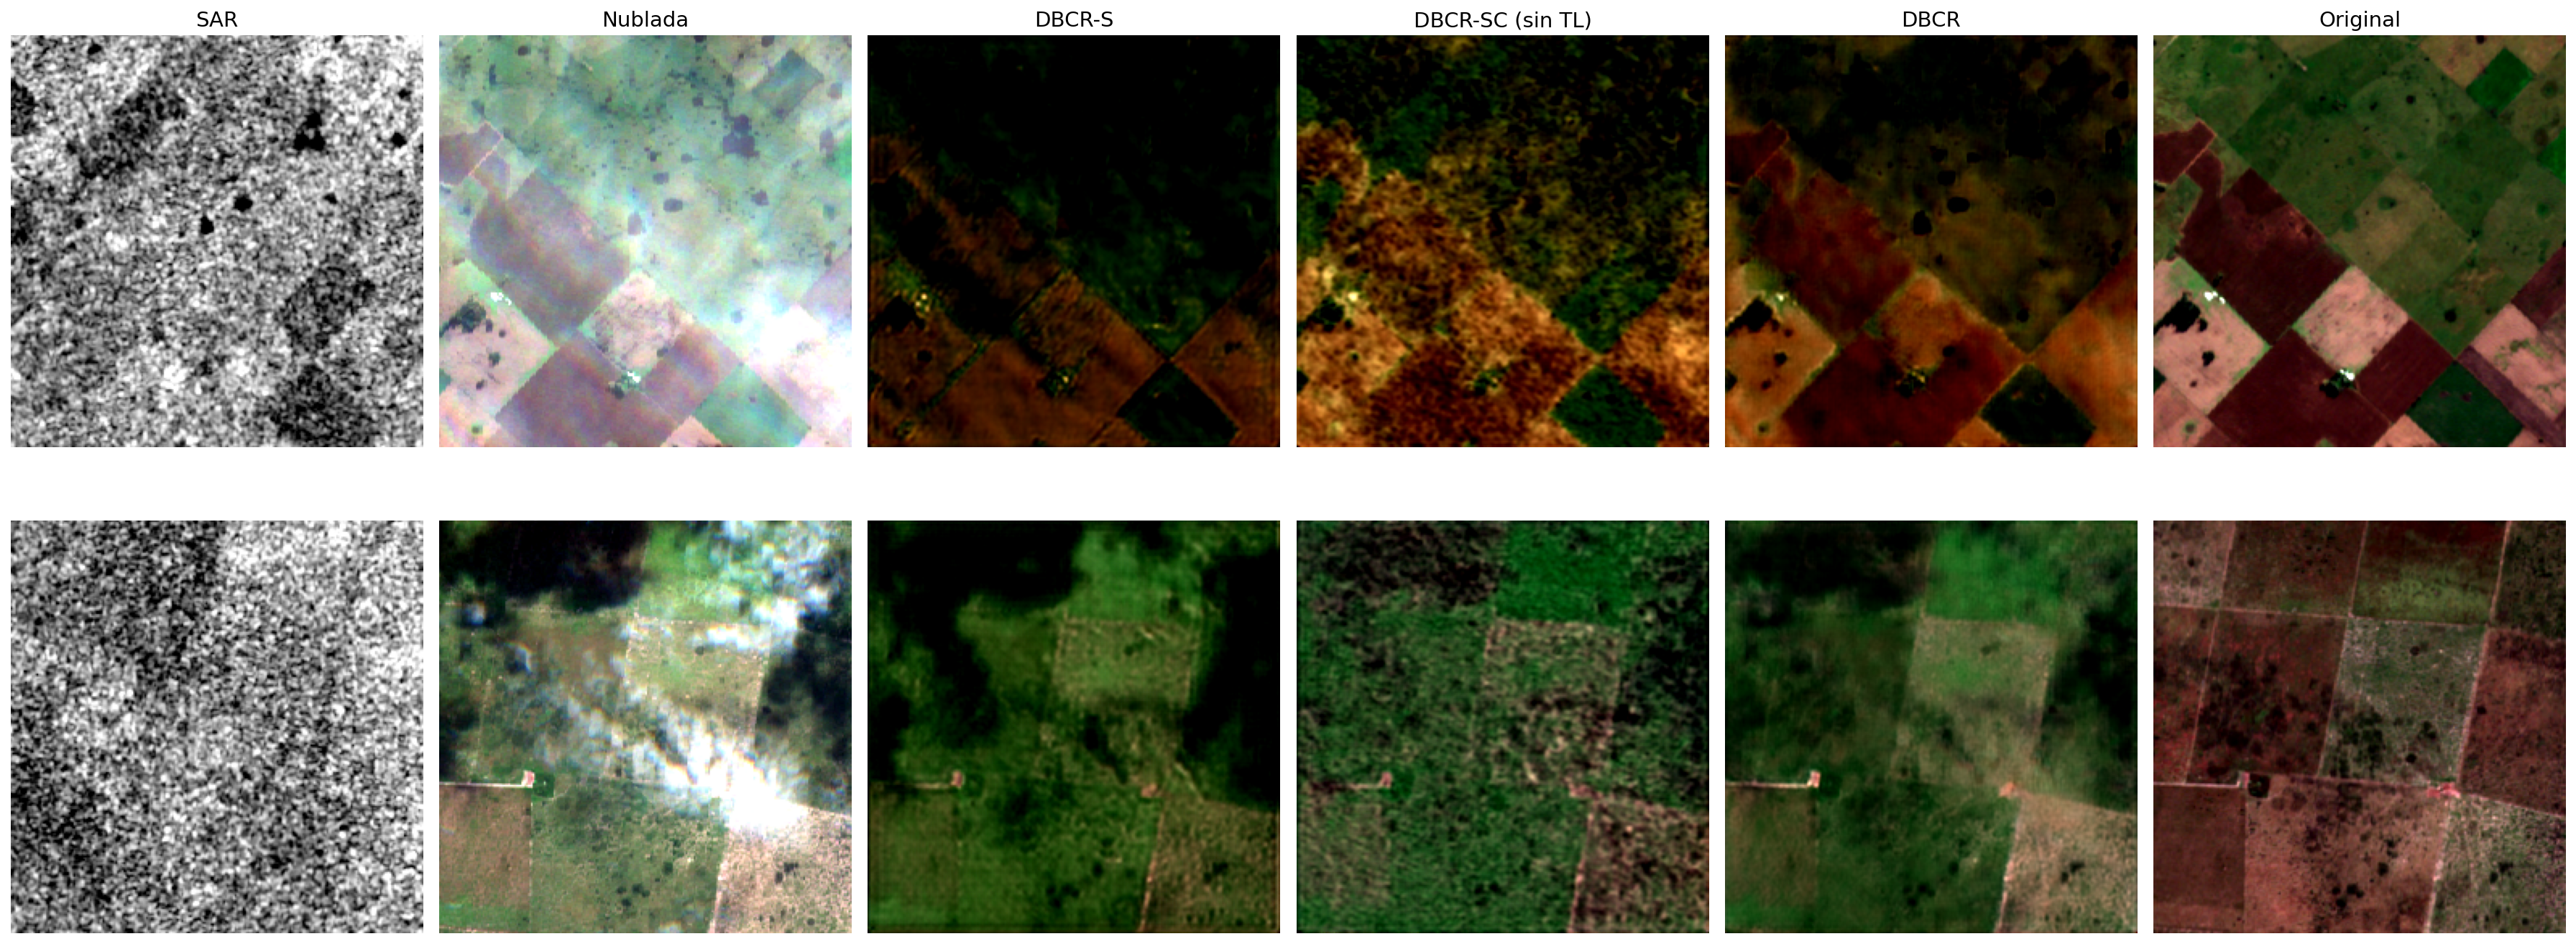
\includegraphics[width=1.0\linewidth]{../imgs/comparacion_modelos.png}
    \caption{Comparación visual sobre dos muestras del conjunto de test. De izquierda a derecha: imagen SAR, imagen nublada, reconstrucciones de DBCR-S, DBCR-SC (sin TL) y DBCR (6 bandas), e imagen de referencia.}
    \label{fig:comparacion_visual}
\end{figure}

Al observar la figura~\ref{fig:comparacion_visual} se visualiza que si bien DBCR-S logra remover las nubes de forma efectiva, tiende a mantener o generar sombras que oscurecen regiones de la imagen que en la reconstrucción original no están presentes. DBCR-SC (sin TL), por su parte, consigue eliminar la cobertura nubosa, pero introduce una textura granular y ruidosa en la reconstrucción. Este efecto es consistente con el hecho de que la concatenación directa incorpora el ruido speckle propio de la señal SAR, sin ningún mecanismo que permita al modelo separarlo, propagándolo hacia la reconstrucción final.

En contraste, DBCR presenta reconstrucciones visiblemente más suaves y sin el sombreado excesivo de DBCR-S, acercándose más a la imagen original en ambos ejemplos. Sin embargo, en la segunda fila puede verse que el modelo no logra eliminar por completo las sombras en la parte superior de la imagen, lo que indica que, si bien el mecanismo de fusión mejora sustancialmente la calidad de la reconstrucción, todavía existen casos donde persisten las sombras.

Estas observaciones sugieren que los bloques SARF permiten aprovechar la información SAR de forma más selectiva que una simple concatenación, logrando una superioridad en calidad visual, permitiendo separar entre información útil y ruido.


% \begin{figure}[H]
%     \centering
%     
\includegraphics[width=0.8\linewidth]{imgs/comparacion_steps_0.png}
%     \caption{Comparación steps}
%     \label{fig:comparacion steps}
% \end{figure}

% Con el fin de ilustrar el efecto de la cantidad de pasos de inferencia sobre la calidad de las imágenes reconstruidas, se presenta en la figura~\ref{fig:comparacion steps} una comparación visual para distintos valores de pasos, evaluada sobre DBCR. Se puede observar que con pocos pasos (e.g., 1--5) las reconstrucciones presentan artefactos y pérdida de detalle, mientras que a partir de los 10 pasos la calidad se estabiliza, con mejoras marginales al aumentar aún más la cantidad. Este comportamiento justifica la elección de 10 pasos como punto de equilibrio entre calidad de reconstrucción y eficiencia computacional.

    \section{Conclusión}
    


% Como posible extensión futura, el bloque SARF podría reemplazar la atención local fija por una variante de deformable cross-attention, donde las features ópticas predigan posiciones relevantes de muestreo sobre las features SAR. Esto permitiría una fusión más adaptativa entre modalidades, manteniendo un costo reducido al atender solo a un conjunto pequeño de puntos relevantes.

% Más experimentos de búsqueda de hiperparámetros, ya sea de redes o de entrenamiento. Agregar validation

% En este trabajo se presenta una aproximación basada en modelos de difusión condicionados para la reconstrucción de imágenes ópticas afectadas por nubes mediante la integración de información SAR y series temporales ópticas. La arquitectura propuesta combina bloques NAFT para el procesamiento óptico-temporal y bloques SARF para la fusión multimodal, además de embeddings temporales que condicionan el proceso generativo.

% Los experimentos realizados sobre el conjunto de datos utilizado muestran que el método es capaz de recuperar estructuras espaciales y texturas relevantes, mejorando la visibilidad de áreas agrícolas y reduciendo artefactos presentes en entradas nubladas. Frente a variantes sin fusión o sin condicionamiento temporal, la propuesta produce reconstrucciones visualmente más coherentes y preserva información espectral útil para posteriores análisis de teledetección.

% Se identifican también limitaciones importantes: la necesidad de una buena co-registración entre SAR y óptico, la sensibilidad al ruido inherente a SAR en ciertas condiciones y la dificultad para reconstruir regiones con oclusión persistente durante largos periodos. Además, la evaluación cuantitativa puede enriquecerse con métricas espectrales y perceptuales adicionales y con pruebas en distintas regiones geográficas y condiciones ambientales.

% Como líneas futuras de trabajo proponemos: (i) mejorar la atención multimodal en el bloque SARF —por ejemplo explorando deformable cross-attention— para una fusión más adaptativa; (ii) realizar una búsqueda sistemática de hiperparámetros y arquitecturas más robustas; (iii) ampliar y diversificar el conjunto de datos y evaluar el método en tareas downstream (clasificación, estimación de índices de vegetación); y (iv) optimizar el coste computacional para facilitar su despliegue operativo.

% En conjunto, los resultados presentan evidencia del potencial de modelos de difusión condicionados multimodales para mitigar el efecto de nubes en imágenes ópticas y para apoyar aplicaciones prácticas de monitoreo remoto.


En este trabajo se implementaron y compararon distintas arquitecturas basadas en modelos difusivos para la tarea de remoción de nubes en imágenes satelitales, con el objetivo de analizar qué formulación difusiva resulta más adecuada para este problema y en qué medida la incorporación de información SAR mejora la reconstrucción óptica.


Respecto del primer punto, los resultados muestran una ventaja clara de la formulación de diffusion bridge frente al DDPM condicional clásico. Mientras que el DDPM debe reconstruir la escena partiendo de ruido gaussiano puro, y no logra estabilizarse ni siquiera al duplicar las épocas de entrenamiento, DBCR-S alcanza un buen desempeño ya a las 15 épocas (PSNR 27.58 dB, SSIM 0.807). Esto confirma la hipótesis que motiva a DB-CR: en cloud removal no resulta óptimo destruir toda la información de la imagen para reconstruirla desde cero, dado que la imagen nublada conserva estructura espacial y espectral aprovechable. Partir de un puente entre la imagen nublada y la limpia define una trayectoria más corta y coherente con la entrada, lo que se traduce en mejor calidad y convergencia más rápida.


Respecto del segundo punto, la evidencia indica que la información SAR aporta mejoras, pero que la forma de fusionarla es determinante. La concatenación directa de canales (DBCR-SC) supera al baseline sin SAR, aunque resulta más efectiva al entrenarse desde el principio que mediante transfer learning, y arrastra el ruido speckle propio del radar hacia la reconstrucción, generando texturas granulares. La estrategia tipo ControlNet (DBCR-SCN), al congelar la rama principal, limita la capacidad del modelo de adaptar sus representaciones internas a la nueva modalidad y no llega a superar a la concatenación simple. Finalmente, la variante con bloques de fusión por atención cruzada (DBCR con SARF Blocks) obtiene el mejor desempeño global (PSNR 28.45 dB, SSIM 0.840, MAE 0.0274), superando tanto al baseline sin SAR como a las demás estrategias de fusión. Esto sugiere que la atención cruzada permite integrar la información radar de forma selectiva, distinguiendo entre contenido útil y ruido, algo que las estrategias más simples no logran. La comparación visual respalda esto: DBCR produce reconstrucciones más suaves, sin el sombreado excesivo de DBCR-S ni la textura ruidosa de DBCR-SC, si bien todavía persisten sombras en algunos casos.


Por otro lado, comparando el mejor modelo de cada configuración, el subconjunto de 6 canales superó al de 13 en las cuatro métricas, lo que indica que las bandas adicionales aportaban principalmente información redundante o de mayor dificultad de ajuste, sin traducirse en una mejor reconstrucción.


Como trabajo futuro, el primer bloque SARF de la arquitectura DBCR podría reemplazar la atención local fija por una variante de deformable cross-attention, en la que las features ópticas predigan las posiciones relevantes de muestreo sobre las features SAR. Esto permitiría una fusión más adaptativa entre modalidades manteniendo un costo acotado, al atender únicamente a un conjunto reducido de puntos relevantes. Asimismo, quedan pendientes una búsqueda de hiperparámetros más exhaustiva, tanto de arquitectura como de entrenamiento, y la incorporación de un conjunto de validación independiente, que en este trabajo no pudo definirse por la limitada cantidad de ROIs disponibles. Finalmente, sería deseable escalar el entrenamiento al dataset SEN12MS-CR completo, en lugar de restringirse a las ROIs de América del Sur, e incorporar técnicas de data augmentation que aumenten la diversidad de las muestras y ayuden a mitigar el posible sobreajuste observado al extender el entrenamiento.
    % \end{multicols}

    \newpage
    \section{Bibliografía}
    1. Ebel, P., Meraner, A., Schmitt, M. & Zhu, X. X. (2020). Multisensor Data Fusion for Cloud Removal in Global and All-Season Sentinel-2 Imagery. IEEE Transactions on Geoscience and Remote Sensing. Disponible en: \url{https://patricktum.github.io/cloud_removal/sen12mscr/}

2. Hu, Y., Lohit, S., Kamilov, U. S. & Marks, T. K. (2025). Multimodal Diffusion Bridge with Attention-Based SAR Fusion for Satellite Image Cloud Removal. arXiv preprint arXiv:2504.03607. Disponible en: \url{https://arxiv.org/pdf/2504.03607}

3. Guo, Z., Lang, J., Huang, S., Gao, Y. & Ding, X. (2025). A Comprehensive Review on Noise Control of Diffusion Model. arXiv preprint arXiv:2502.04669. Disponible en: \url{https://arxiv.org/pdf/2502.04669}

4. Zou, X., Li, K., Xing, J., Zhang, Y., Wang, S., Jin, L. & Tao, P. (2023). DiffCR: A Fast Conditional Diffusion Framework for Cloud Removal from Optical Satellite Images. arXiv preprint arXiv:2308.04417. Disponible en: \url{https://arxiv.org/pdf/2308.04417}

5. Chen, L., Chu, X., Zhang, X. & Sun, J. (2022). Simple Baselines for Image Restoration. arXiv preprint arXiv:2204.04676. Disponible en: \url{https://arxiv.org/pdf/2204.04676}

6. Zhang, L., Rao, A. & Agrawala, M. (2023). Adding Conditional Control to Text-to-Image Diffusion Models. arXiv preprint arXiv:2302.05543. Disponible en: \url{https://arxiv.org/pdf/2302.05543}

7. Liu, Z., Lin, Y., Cao, Y., Hu, H., Wei, Y., Zhang, Z., Lin, S. & Guo, B. (2021). Swin Transformer: Hierarchical Vision Transformer using Shifted Windows. arXiv preprint arXiv:2103.14030. Disponible en: \url{https://arxiv.org/pdf/2103.14030}

8. Wang, Z., Bovik, A. C., Sheikh, H. R. & Simoncelli, E. P. (2004). Image Quality Assessment: From Error Visibility to Structural Similarity. IEEE Transactions on Image Processing, 13(4), 600--612. Disponible en: \url{https://ece.uwaterloo.ca/~z70wang/publications/ssim.pdf}

9. Kruse, F. A., Lefkoff, A. B., Boardman, J. W., Heidebrecht, K. B., Shapiro, A. T., Barloon, P. J. & Goetz, A. F. H. (1993). The Spectral Image Processing System (SIPS) -- Interactive Visualization and Analysis of Imaging Spectrometer Data. Remote Sensing of Environment, 44(2-3), 145--163. Disponible en: \url{https://ui.adsabs.harvard.edu/abs/1993RSEnv..44..145K/abstract}

10. Chen, T., Xu, B., Zhang, C. & Guestrin, C. (2016). Training Deep Nets with Sublinear Memory Cost. arXiv preprint arXiv:1604.06174. Disponible en: \url{https://arxiv.org/pdf/1604.06174}

11. Dao, T., Fu, D. Y., Ermon, S., Rudra, A. & Ré, C. (2022). FlashAttention: Fast and Memory-Efficient Exact Attention with IO-Awareness. arXiv preprint arXiv:2205.14135. Disponible en: \url{https://arxiv.org/pdf/2205.14135}

12. PyTorch (2025). Automatic Mixed Precision Package -- torch.amp (Autocast). Documentación oficial de PyTorch, versión 2.12. Disponible en: \url{https://docs.pytorch.org/docs/2.13/amp.html}

    % % \newpage
    % \input{8.tabla}
\end{document}